\section{Pebble Damage Modeling}\label{sec:failure-study}

It is impractical, if not impossible, to experimentally measure accurate contact forces between all the pebbles in a densely-packed, three-dimensional ensemble. In investigating the probability of pebbles becoming damaged (\textit{i.e.} crushed or cracked) in a packed bed, we therefore rely on the combined information gained from indirect measurements of the entire pebble bed, crush experiments of individual pebbles, and the predictive capabilities of DEM simulations. In this section I first employ observations of individual pebble crush experiments to create a metric (strain energy) to link the data to the contact forces measured in DEM to help predict when pebbles in the ensemble will become damaged. I then review some literature where similar efforts have been performed at other research institutions and point out why the method employed here is preferred. Finally I show some numerical recipes I have developed for modeling the fragmentation event of a crushed pebble in the DEM framework -- along with an evaluation of some fragmentation schemes. 

\subsection{Experimental Measurements of Strain Energy}
\begin{figure}[!t]
\centering
    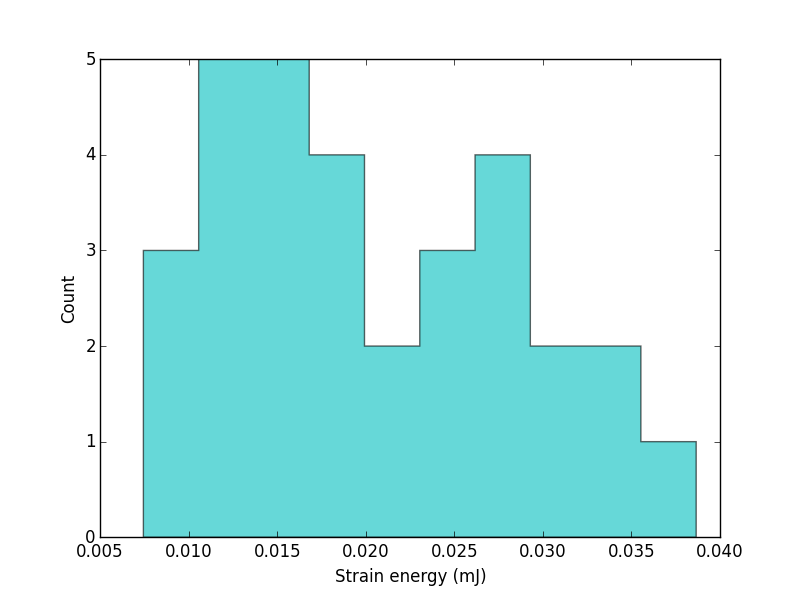
\includegraphics[width=\doubleimagewidth]{chapters/figures/fzk-w-histogram.png}
    \caption{Histogram of the absorbed strain energy at the moment of crushing for \lis~pebbles as measured in single pebble crush experiments.}
    \label{fig:fzk-w-hist}
\end{figure}

\begin{figure}
        \centering
        \begin{subfigure}[b]{\doubleimagewidth}
                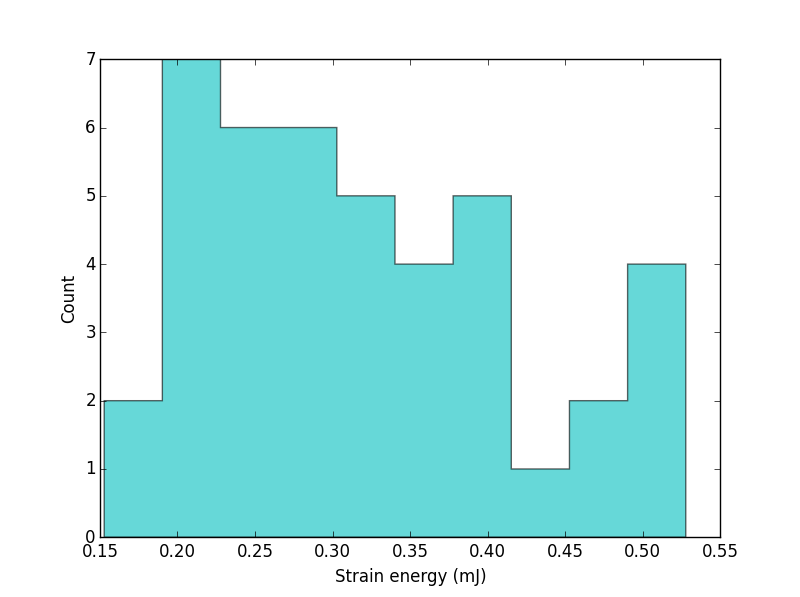
\includegraphics[width=\textwidth]{chapters/figures/nfri-1mm-w-histogram.png}
                \caption{$\bar{d}_p = 1$ mm}
                \label{fig:nfri-1-w-hist}
        \end{subfigure}
        ~
        \begin{subfigure}[b]{\doubleimagewidth}
                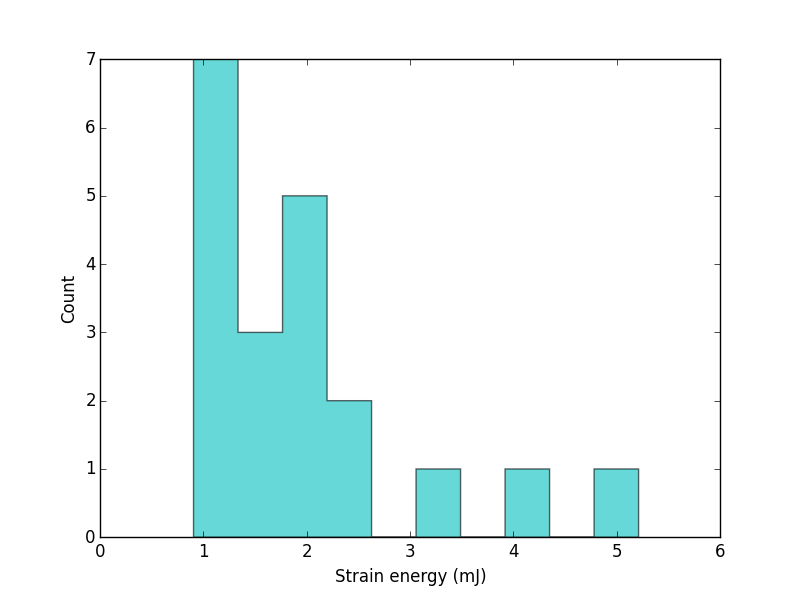
\includegraphics[width=\textwidth]{chapters/figures/nfri-1.5mm-w-histogram.png}
                \caption{$\bar{d}_p = 1.5$ mm}
                \label{fig:nfri-1.5-w-hist}
        \end{subfigure}
        \caption{Histogram of the absorbed strain energy at the moment of crushing for \lit~pebbles as measured in single pebble crush experiments.}\label{fig:nfri-w-hist}
\end{figure}

The normal force between two elastic objects is a function of the material properties of the interacting objects (see, \textit{e.g.}, Eq.~\ref{eq:hertz-normal-force}). We cannot, therefore, directly compare the forces between the pebble and test stand with pebble-pebble contacts in an ensemble. An approached used by some solid breeder researchers is to relate the total absorbed strain energy of the pebble.\cite{Zhao2013,Annabattula2012a}

Integrating the Hertzian force along the overlap of contact to find the strain energy $W_\epsilon$, of a given contact,
\begin{equation}\label{eq:strain-energy-integral}
	W_\epsilon = \int_0^{\delta_c}\!F_n(\delta')\,\mathrm{d}\delta'
\end{equation}
where the upper limit of the integration is the critical overlap $\delta_c$. Inserting the Hertzian relation of Eq.~\ref{eq:hertz-normal-force} into Eq.~\ref{eq:strain-energy-integral} gives,
\begin{align}
	W_\epsilon& = \int_0^{\delta_c}\!  \frac{4}{3}E^*\sqrt{R^*}\,\delta'^{3/2} \,\mathrm{d}\delta' \\
	%W_\epsilon & = \frac{4}{3}E^*\sqrt{R^*} \left[\frac{2}{5}\,{\delta_c}^{5/2}\right] \\
	W_\epsilon & = \frac{8}{15}E^*\sqrt{R^*}\, {\delta_c}^{5/2}
\end{align}

I will call the strain energy of the pebble compressed between platens as the lab strain energy, $W_{\epsilon,L}$. In pebble crushing experiments, we record the strain energy absorbed up to the point of crushing, the data for \lis~and \lit~pebbles are shown in Figs.~\ref{fig:fzk-w-hist} and~\ref{fig:nfri-w-hist}, respectively. The strain energy of two particles in contact will be $W_{\epsilon,B}$. The assumption is made that, if each contact interaction is integrated to the proper critical overlap, the strain energies will be equal at that contact. The critical lab value is equated to the ensemble value,
\begin{equation}
	W_{\epsilon,L} = W_{\epsilon,B} = \frac{8}{15}E_B^*\sqrt{R_B^*}\, {\delta_{c,B}}^{5/2}
\end{equation}
which allows one to solve for the interacting pebble bed overlap as a function of the lab strain energy,
\begin{equation}
	\delta_{c,B} = \left[\frac{15W_{\epsilon,L}}{8E_B^*\sqrt{R_B^*}}\right]^{2/5}
\end{equation}

This overlap can be reinserted to the Hertz force of Eq.~\ref{eq:hertz-normal-force} to find the critical force (crush force) of the interacting particles in the numeric ensemble as a function of the critical strain energy of the lab. Doing this, we find,
\begin{equation}\label{eq:peb_hertz}
	F_{c,B} = C{E_B^*}^{2/5}{R_B^*}^{1/5}W_{\epsilon,L}^{3/5}
\end{equation}
where $C = \frac{4}{3}\left(\frac{15}{8}\right)^{3/5}$.

Equation~\ref{eq:peb_hertz} is a generic translation between lab materials and packed bed materials. We will use the equation as the basis for our pebble crushing prediction in DEM simulations. Before implementing a custom crush-predicting method into the DEM code, I will review other attempts at modeling and predicting crush behavior in packed beds.





% FROM SOFT PAPER
\subsection{Calculating Critical Strain Energy}
With the rise of micro-mechanical tools and computing power, attempting to predict when ceramic pebbles will crush in an ensemble, based on inter-particle contact forces, has received considerable attention. In this section I review literature studying granular crushing.

Probability and statistics were applied to the study of packed beds of brittle grains by Marketos and Bolton\cite{Marketos2007}. The fundamental assumption in their predictive method was the independence of crushing events. They used their model to predict the initiation of crushing as well as the evolution of the packing after crushing. They created somewhat arbitrary probability distributions of the strength of their granular particles,
\begin{equation}
	h(\Phi) = \frac{0.0395}{\sqrt{\Phi}}
\end{equation}
where $\Phi$ is a characteristic strength parameter falling between 160 and 640~N. The form of their distribution was based on single crushing tests on quartz particles from Nakata\etal.

A common alternative distribution is to use a form first proposed by Weibull for a material under uniform stress\cite{Kwok2013,Zhao2011,nakata1999probabilistic,Zhao2013,Pitchumani2004}. The form, as written by Zhao\etal~is,
\begin{equation}
	P_s = 1 - \exp\left[-\left(\frac{W_c}{W_\text{mat}}\right)^m\right]
\end{equation}
where $W_c$ is the energy absorbed by the pebble and $W_\text{mat}$ and $m$ characterize the material. An important note is how to calculate the critical strain energy for the pebble. Refs.~\cite{Marketos2007} and \cite{Zhao2011} note the necessity to consider the coordination number dependence on total strain energy. In other words, the total strain energy is the cumulative total of strain energy at every contact. Zhao\etal~give the critical strain as
\begin{equation}
	W_c = \sum_{i=1}^{Z_i}\left(\frac{9}{80 R_{ij}^*}\right)^{1/3} \left(\frac{1}{E_{ij}^*}\right)^{2/3} F_{n,ij}^{5/3}
\end{equation}
where $Z$ is the coordination number of pebble $i$. 

However, Russell\etal, analyzed simple, ideal granular assemblies for which they could find analytical solutions to stress distributions inside of pebbles.\cite{Russell2009} In their work, failure of a granular particle initiates at the location of maximum of the stress invariant ratios. In the contact of elastic spheres, the stress fields near the contact areas are highly localized. Because of the highly localized effects, Russell\etal~find that in granular assemblies the contributions to failure initiation are not additive. They discovered that the initiation of failure is always located adjacent to the largest force irrespective of the material properties or geometric size of the pebbles in an ensemble. Russell\etal conclude: \emph{the largest contact force acting upon a particle is the primary agent driving the damage of the individual}.\cite{Russell2009} Based upon the failure criterion developed for brittle materials, crushing of an individual does not directly depend upon the presence or magnitude of any lesser contact forces acting on the particle or the material properties of the particle. Although their results were obtained for idealized assemblies, the results are generally true for any situation where multiple contact forces are present.

\begin{figure}[!t]
\centering
    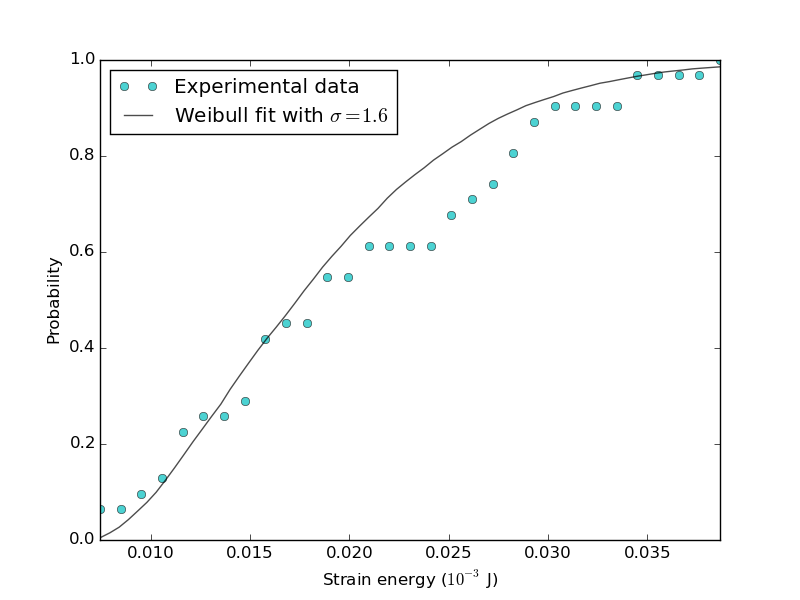
\includegraphics[width=\doubleimagewidth]{chapters/figures/fzk-w-cdf-fit.png}
    \caption{Fitting the strain energy with a Weibull distribution with shape parameter specific for the \lis~pebbles.}
    \label{fig:fzk-w-cdf}
\end{figure}

\begin{figure}
        \centering
        \begin{subfigure}[b]{\doubleimagewidth}
                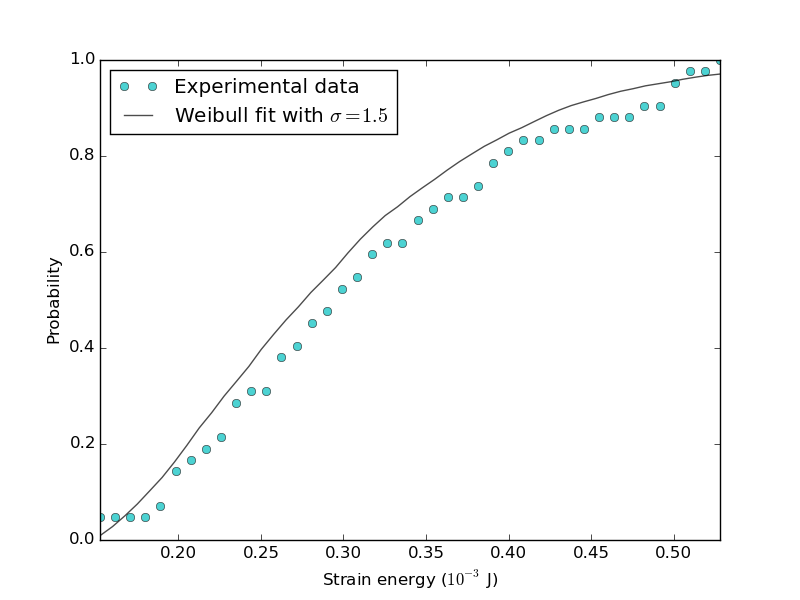
\includegraphics[width=\textwidth]{chapters/figures/nfri-1mm-w-cdf-fit.png}
                \caption{$\bar{d}_p = 1$ mm}
                \label{fig:nfri-1-w-cdf}
        \end{subfigure}
        ~
        \begin{subfigure}[b]{\doubleimagewidth}
                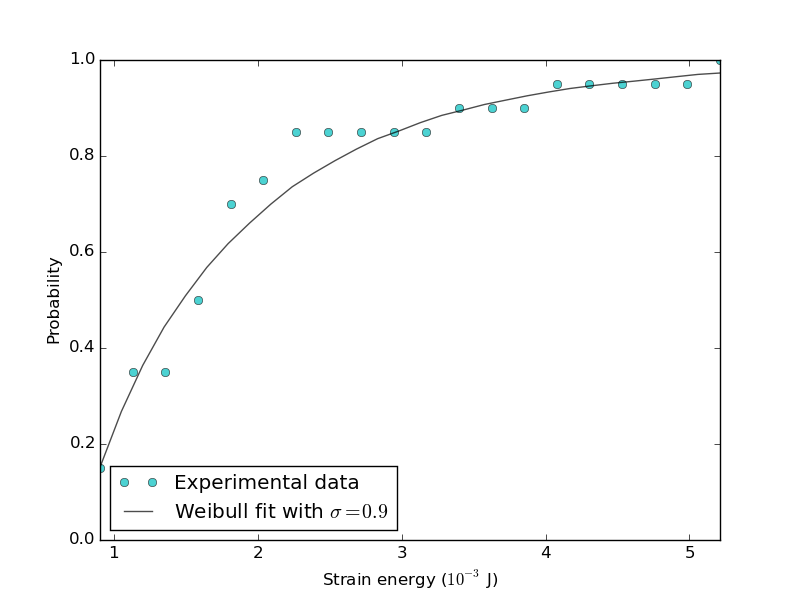
\includegraphics[width=\textwidth]{chapters/figures/nfri-1.5mm-w-cdf-fit.png}
                \caption{$\bar{d}_p = 1.5$ mm}
                \label{fig:nfri-1.5-w-cdf}
        \end{subfigure}
        \caption{Fitting the strain energy with a Weibull distribution with shape parameter specific for the two batches of \lit~pebbles.}\label{fig:nfri-w-cdf}
\end{figure}

Based on the compelling arguments of Russell\etal, I define a critical force as the maximum contact force on the pebble in our assembly,
\begin{equation}
	F_{c} = \max F_{n,ij}
\end{equation}

Then define a pebble crushing event as occurring when \textit{any} force on the pebble in the bed is greater than the critical bed force defined from Eq.~\ref{eq:peb_hertz},
\begin{equation}\label{eq:crush-predict}
  F_{c} > F_{c,B} = \frac{4}{3}\left(\frac{15}{8}\right)^{3/5}{E_B^*}^{2/5}{R_B^*}^{1/5}W_{\epsilon,L}^{3/5}
\end{equation}

In the implementation into DEM, the probabilistic features appear naturally in this formulation from the measured $W_{\epsilon,L}$ of experiments. This value follows a probability distribution and therefore imparts a distribution shape to the $F_{c,B}$ prediction. Cumulative distribution functions are generated for the strain energy data (see Fig.~\ref{fig:nfri-w-hist}). From that data, we fit Weibull distribution curves, of the form
\begin{equation}
	\Xi = \lambda\left[-\ln(W_\epsilon)\right]^{1/\sigma}
\end{equation}
where the shape parameter, $\sigma$, is fit to the specific curve of each set of experimental data and the second parameter, $\lambda$ is defined as
\[
\lambda = \bar{W}_\epsilon - \min W_\epsilon
\]

In Figs.~\ref{fig:fzk-w-cdf} and~\ref{fig:nfri-w-cdf} we see the experimental data and the Weibull fits specific to the ceramic material and batch. The Weibull distribution functions are recreated numerically in the assignment of each pebbles `critical bed force' value.


% \cite{Hiramatsu1966}
% From , 
% \begin{align*}
% \sigma_{cr} = \cfrac{2.8}{\pi}\cfrac{F_{cr}}{4R^2}
% \end{align*}
Research on pebble damage has been taken up by others in the fusion community to predict the onset of pebble crushing as a function of an external pressure and the resulting changes to mechanical properties such as the stress-strain of the pebble bed.\cite{Annabattula2012a, Zhao2012, Zhao2013} Other fields of engineering have also employed DEM in studies of granular crushing with generally similar modeling approaches.\cite{Marketos2007,Pitchumani2004}


In modeling pebble damage, there are two main tasks: predicting when the grain crushes and what happens to the pebble during the crushing event. For the former, the task is to develop a model for predicting a pebble crushing event; \textit{i.e.} what external load (mechanical or thermal) will cause a pebble to crack, shatter, fracture, etc. To tackle the latter is to develop a model which simulates the damage of that pebble; \textit{i.e.} a scheme to treat a cracked, shattered, or crushed pebble in the assembly as small particles, removed particles, or particles with modified material properties.

\begin{figure}[!t]
\centering
	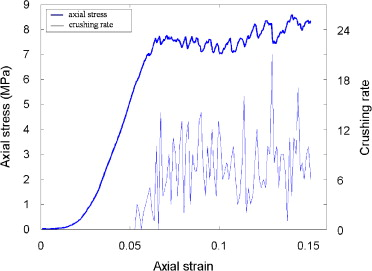
\includegraphics[width=\singleimagewidth]{chapters/figures/markets-bolton-stress-strain-crushing.jpg}
	\caption{Stress-strain response of a pebble bed with crushed pebbles. Reproduced from Ref.~\cite{Marketos2007}}
	\label{fig:marketos-bolton-stress-strain}
\end{figure}

\begin{figure}[!t]
\centering
	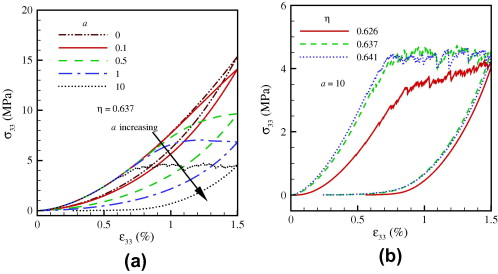
\includegraphics[width=\singleimagewidth]{chapters/figures/annabattula-stress-strain-crushing.jpg}
	\caption{Stress-strain response of a pebble bed with crushed pebbles. Reproduced from Ref.~\cite{Annabattula2012a}}
	\label{fig:annabattula-stress-strain}
\end{figure}

The numerical study to follow will focus on the `what happens' question. In work by Marketos and Bolton, they treated a crushed pebble very similar to Van Lew\etal; when a pebble was damaged it was removed completely from the assembly.\cite{Marketos2007,VanLew2014} Marketos and Bolton study the stress-strain response of a pebble bed with a predictive crushing routine while Van Lew\etal~studied the effective thermal conductivity of a damaged pebble bed.

However, in the case of Van Lew\etal, the technique of removing a pebble is limited by the fact that energy input into two systems being studied is not comparable. Because of volumetric energy deposition in the simulations, the total energy pouring into the non-damaged system would be
\begin{equation}
	E_h = \frac{q'''_\text{nuc} V_\text{peb} N}{V_\text{bed}}
\end{equation}
where $N$ is the total number of pebbles of volume $V_\text{peb}$ that exist in the pebble bed of volume $V_\text{bed}$. After a crushing event, when pebbles are removed, the total amount of energy is
\begin{equation}
	E_h' = \frac{q'''_\text{nuc} V_\text{peb} \eta N}{V_\text{bed}}
\end{equation}
where $\eta$ is the percent of crushed pebbles. Obviously then, the ratio of the two heating rates is\begin{equation}
	\frac{E_h'}{E_h} = 1 - \eta
\end{equation}
and the energy deposited is not balanced between a virgin bed and one with crushed pebbles. We will attempt to address this issue.

\subsection{Modeling Fragments of a Crushed Pebble}\label{sec:fragmentation}
In the DEM framework, we are limited to modeling elastic spheres. If we strictly wish to conserve mass between a solid pebble of radius $R_p$ and the crushed fragments of radius $R_c$, then the number of crushed fragments (spheres) per crushed pebble is
\begin{equation}\label{eq:nc-crushed-fragments}
	N_c = \left(\frac{R_c}{R_p}\right)^{-3}
\end{equation}

Thus the number of fragments goes like the inverse of radius ratio to the third power and the number of crushed fragments to represent a single crushed pebble increases rapidly as the fragments shrink. The relationship between radius ratio and number of fragment particles is given in Fig.~\ref{fig:fragment-count}. Note that in the DEM simulation, it is impossible to insert fractions of a particle so the number of fragment pebbles is rounded to the nearest integer in the figure.


\begin {table}[htp] %
\caption{Example values of the particle crush fragments, $N_c$, necessary to replace a single crushed particle and obey conservation of mass (fragment number is rounded to nearest integer).}
\label {tab:rstar-Nc} \centering %
\begin {tabular}{ S[table-format=3.2]S[table-format=3.2] }
\toprule
$R_c/R_p$ 						& $N_c$  				\\\otoprule
0.20                            & 125                   \\    
0.30                            & 37               \\
0.40                            & 16                   \\
0.50                            & 8                         \\
0.75                            & 2                \\\bottomrule
\end{tabular}
\end{table}



\begin{figure}[!t]
\centering
    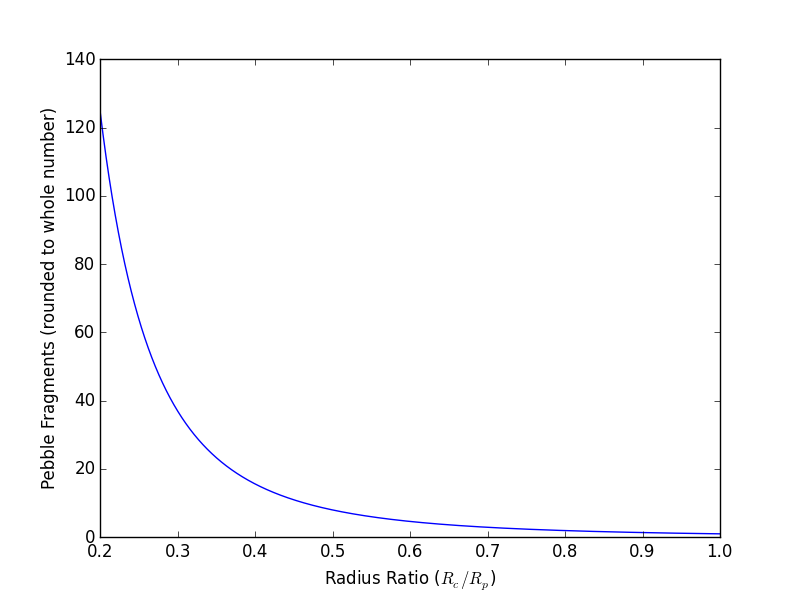
\includegraphics[width=\singleimagewidth]{chapters/figures/crush-fragments/pebble-fragment-count.png}
    \caption{Number of fragment pebbles necessary to conserve mass increases rapidly as the size of the radius ratio ($\frac{R_c}{R_p}$) decreases.}
    \label{fig:fragment-count}
\end{figure}

In typical DEM simulations that can run within reasonable amounts of time on the machines available for this dissertation, a reasonable number of particles is on the order of \num{10000}. Significantly more and the run times become impractical for study. To show how quickly the number of particle fragments can quickly get out of hand in a simulation with small $R_c/R_p$, if we begin with \num{6000} pebbles and only 2\% break, with a radius ratio of $R_c/R_p = 0.2$, the number of pebbles to be added would be \num{15000}. The new particle fragments (less the crushed particles) plus the original would require \num{21000} particles in the system. In our simulations, we often test the effects on effective thermal conductivity at particle crush amounts of to 10\%. For the pebble bed mentioned here, that would mean \num{81000} particles in the system and it would be computationally taxing. The result is that, for the sake of computational times, the larger crush fragment radii are desired, \textit{i.e.} $R_c/R_p > 0.3$.

However, aside from satisfying conservation of mass, we must physically insert the particle fragments into void space in the simulation domain. During the course of the simulation, when we choose to replace the pebble with the fragments, the only available room is the spherical void left over by the damaged pebble. Thus a constraint is the smallest sized sphere that will allow the given spheres at most dense packing. 

Dense packing of spheres inside a larger sphere is an interesting mathematical problem. \href{http://www.randomwalk.de/sphere/insphr/spisbest.txt}{Hugh Pfoertner} keeps a compiled list of many solutions for a number of particles; many solutions are his are from Gensane.\cite{gensane2003dense} If we consider, for instance, that a radius ratio of $R_c/R_p = 0.3$ requires 37 particle fragments, then we can also find from Ref.~\cite{gensane2003dense} that 37 particles would have to be of radius 0.2406866 to fit into a single sphere of radius of unity. We defined the particle fragment radius as $R_c$, the original particle as $R_p$, and then the radius of sphere necessary to hold the $N_c$ fragments will be $R_N$, we can find a relationship between the volume of sphere $V_p$ and necessary volume $V_N$,
\begin{equation}
	r_1^* = \frac{R_c}{R_p}
\end{equation}
and
\begin{equation}
	r_2^* = \frac{R_c}{R_N}
\end{equation}
then 
\begin{equation}
	R_N = R_p \frac{r_1^*}{r_2^*}
\end{equation}
thus
\begin{equation}
	\frac{V_N}{V_p} = \left(\frac{r_1^*}{r_2^*}\right)^3
\end{equation}

If we choose a linearly spaced distribution of $r_1^*$ between 0 and 1, we can then find how many $N_c$ particles are necessary to conserve mass, then from the $N_c$ particles we can find from the database of sphere packing solutions the size of sphere that would be necessary to fit the $N_c$ particles. The calculations are carried out and shown in Fig.\ref{fig:volume-ratio}. The data in Ref.~\cite{gensane2003dense} does not go above 72 spheres so we are limited to radius ratios above about $r_1^* > 0.24$.

The plot of Fig.\ref{fig:volume-ratio} shows that for particle fragments of reasonable numbers ($N_c\approx 20$ for $r_1^*\approx 0.3$), the volume necessary to fit the number of volume-conserving particles is greater than double the volume of the original sphere! Therefore from the point of view of having the physical space to insert the fragments, smaller sized fragments are ideal. To insert the few number of large particles would require disrupting the packing in the region of the damaged particle.

Thus we have competing results from the two requirements. Computationally, we desire larger crushed fragments yet we need smaller fragments in order to fit them into the system in a non-disruptive way.

\begin{figure}[!t]
\centering
    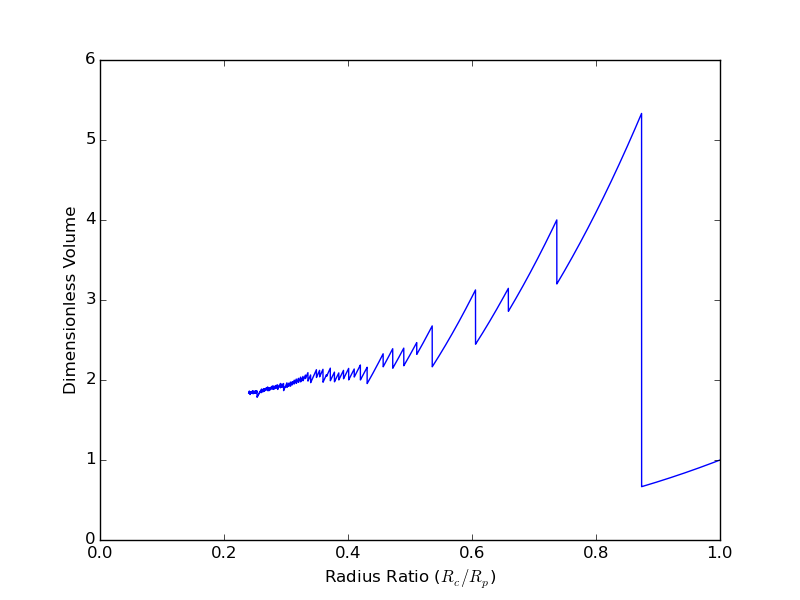
\includegraphics[width=\singleimagewidth]{chapters/figures/crush-fragments/fragment-volume-ratio.png}
    \caption{The volume necessary to house the particles of different radius ratios decreases toward unity as the radius ratio decreases. It is greater than 5 times the volume for large $r_1^*$.}
    \label{fig:volume-ratio}
\end{figure}




\begin{figure}[!ht]
	\centering
	\begin{subfigure}[b]{\doubleimagewidth}
		\centering
		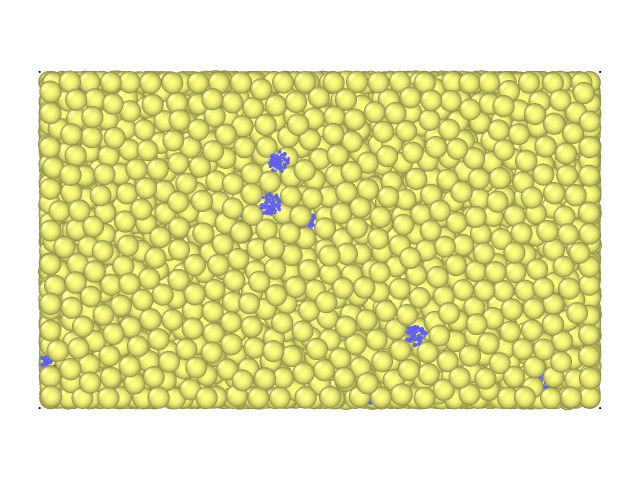
\includegraphics[width=\textwidth]{chapters/figures/crush-fragments/0.20-1.png}
		\caption{initial}
	\end{subfigure}
	\begin{subfigure}[b]{\doubleimagewidth}
		\centering
		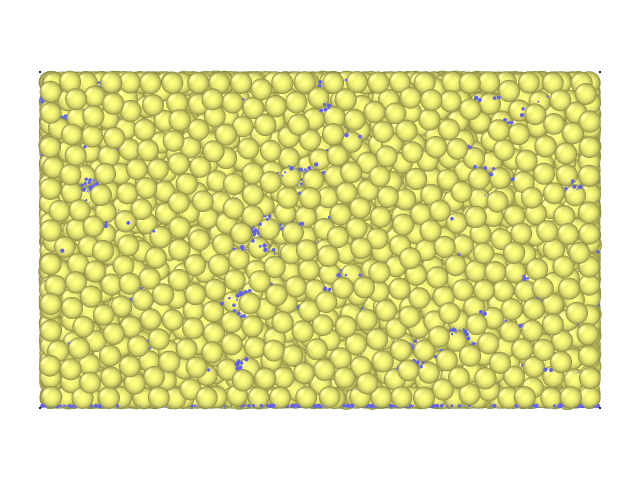
\includegraphics[width=\textwidth]{chapters/figures/crush-fragments/0.20-2.png}
		\caption{final}
	\end{subfigure}
	\caption{$N_c = 8594$, $N_\text{tot} = 15430$, $r_1^* = 0.20$. Side view of the packing arrangement and settling for different crush fragment sizes. The small crush fragments migrate far through the height of the bed. The yellow particles are the original pebbles and the blue are fragments inserted into the system after pebble crushing.}
\label{fig:crush-settling-pictures-1}
\end{figure}
\begin{figure}[!ht]
	\begin{subfigure}[b]{\doubleimagewidth}
		\centering
		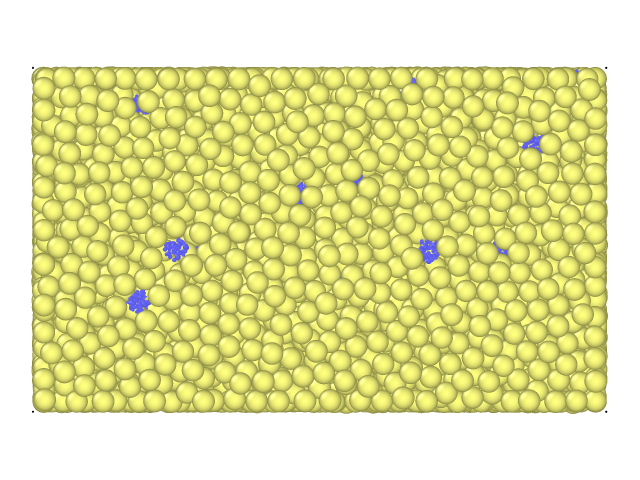
\includegraphics[width=\textwidth]{chapters/figures/crush-fragments/0.25-1.png}
		\caption{initial}
	\end{subfigure}
	\begin{subfigure}[b]{\doubleimagewidth}
		\centering
		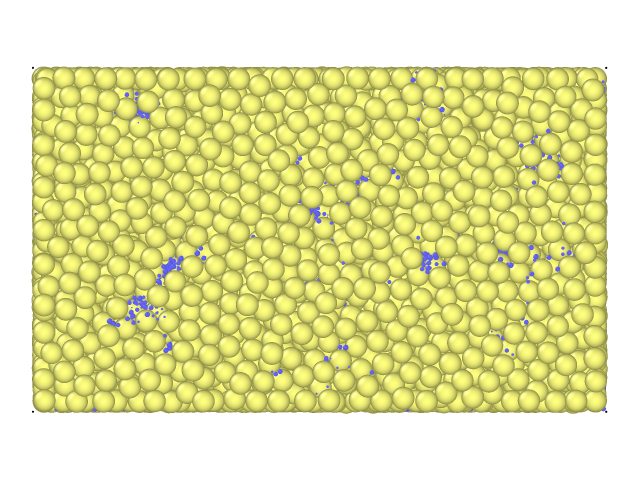
\includegraphics[width=\textwidth]{chapters/figures/crush-fragments/0.25-2.png}
		\caption{final}
	\end{subfigure}
	\caption{$N_c = 4400$, $N_\text{tot} = 11222$, $r_1^* = 0.25$. Side view of the packing arrangement and settling for different crush fragment sizes. The small crush fragments migrate far through the height of the bed. The yellow particles are the original pebbles and the blue are fragments inserted into the system after pebble crushing.}
\label{fig:crush-settling-pictures-2}
\end{figure}

\begin{figure}[!ht]
	\centering
	\begin{subfigure}[b]{\doubleimagewidth}
		\centering
		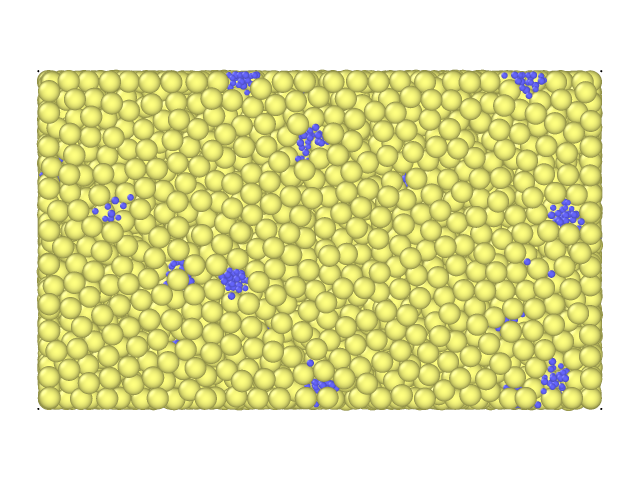
\includegraphics[width=\textwidth]{chapters/figures/crush-fragments/0.35-1.png}
		\caption{initial}
	\end{subfigure}
	\begin{subfigure}[b]{\doubleimagewidth}
		\centering
		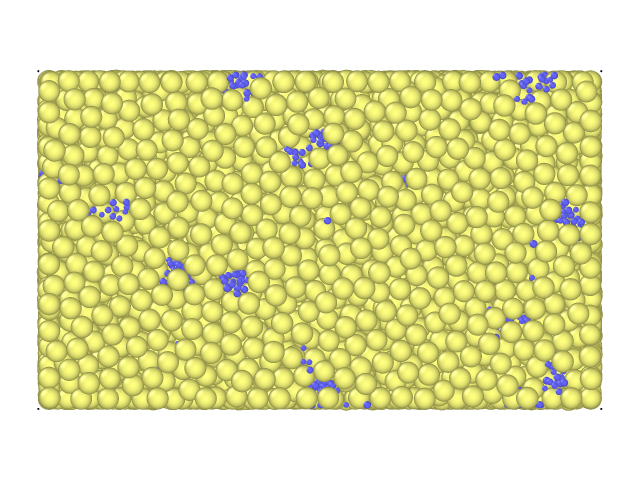
\includegraphics[width=\textwidth]{chapters/figures/crush-fragments/0.35-2.png}
		\caption{final}
	\end{subfigure}
	\caption{$N_c = 1603$, $N_\text{tot} = 8393$, $r_1^* = 0.35$. Side view of the packing arrangement and settling for different crush fragment sizes. The bigger fragments remain largely in place. The yellow particles are the original pebbles and the blue are fragments inserted into the system after pebble crushing.}
\label{fig:crush-settling-pictures-3}
\end{figure}
\begin{figure}[!ht]
	\begin{subfigure}[b]{\doubleimagewidth}
		\centering
		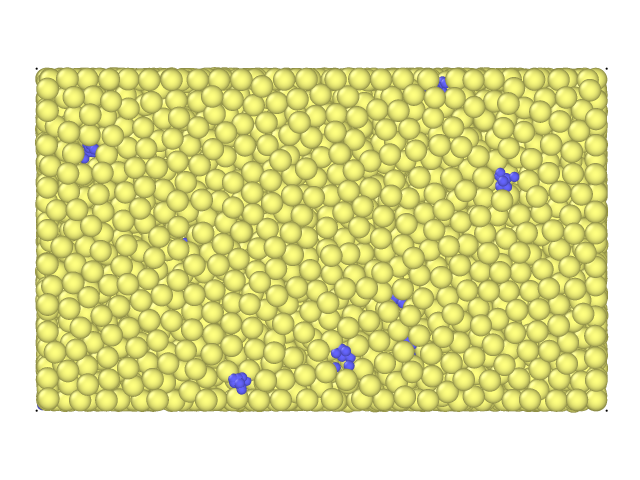
\includegraphics[width=\textwidth]{chapters/figures/crush-fragments/0.50-1.png}
		\caption{initial}
	\end{subfigure}
	\begin{subfigure}[b]{\doubleimagewidth}
		\centering
		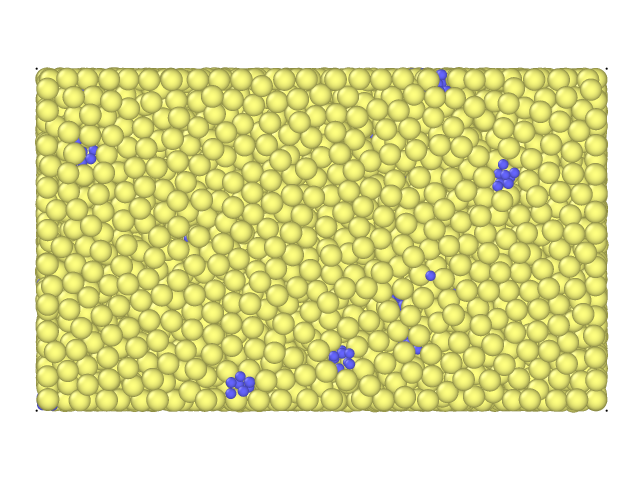
\includegraphics[width=\textwidth]{chapters/figures/crush-fragments/0.50-2.png}
		\caption{final}
	\end{subfigure}
	\caption{$N_c = 550$, $N_\text{tot} = 7358$, $r_1^* = 0.50$. Side view of the packing arrangement and settling for different crush fragment sizes. The bigger fragments remain largely in place. The yellow particles are the original pebbles and the blue are fragments inserted into the system after pebble crushing.}
\label{fig:crush-settling-pictures-4}
\end{figure}
\FloatBarrier

To study the effects on a pebble bed of different fragmentation schemes, I begin with a bed of \num{6875} particles and randomly crush 1\%. This was done with a range of fragments of size $r_1^* = [0.20, 0.25, 0.35, 0.50]$. The number of particles inserted for these different $r_1^*$ followed the from Eq.~\ref{eq:nc-crushed-fragments}. In the images of Figs.~\ref{fig:crush-settling-pictures-1},~\ref{fig:crush-settling-pictures-2},~\ref{fig:crush-settling-pictures-3}, and~\ref{fig:crush-settling-pictures-4}, we see the initial packing of new particle fragments (in blue) settle into the interstitial gaps of the packing structure of original pebbles (yellow).

\begin{figure}[!t]
\centering
    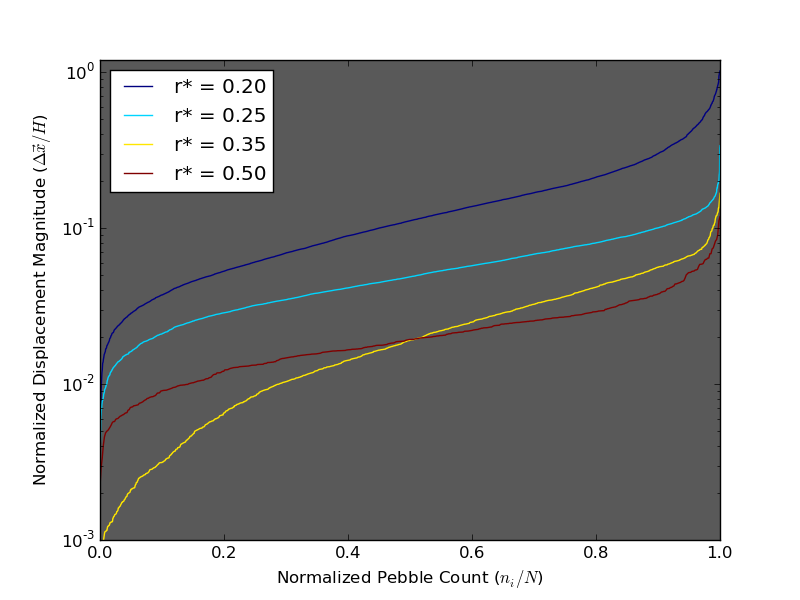
\includegraphics[width=\singleimagewidth]{chapters/figures/crush-fragments/displacement-scatter-radius-ratios.png}
    \caption{After the particle fragments are inserted into the system they re-settle due to gravity and inter-particle forces. The small fragments travel much further throughout the bed than the large fragments.}
    \label{fig:displacement-scatter}
\end{figure}

The settling of crushing fragments is also visualized in Fig.~\ref{fig:displacement-scatter}. For this figure, the magnitude of displacement for all the crushed fragments is recorded based on the change between initial insertion location and final resting place. The displacement of the fragments is normalized against the height of the pebble bed, $H$. The fragments with $r_1^* = 0.2$ are seen to travel, on average, 10\% of the height of the pebble bed before coming to rest; some of them travel more than the entire height of the bed -- as if in a game of Plinko. In contrast, the particle fragments of size $r_1^* = 0.35$ and $r_1^* = 0.5$ travel only about 1\% of the height of the bed before coming to rest. 

\begin{figure}[!t]
\centering
    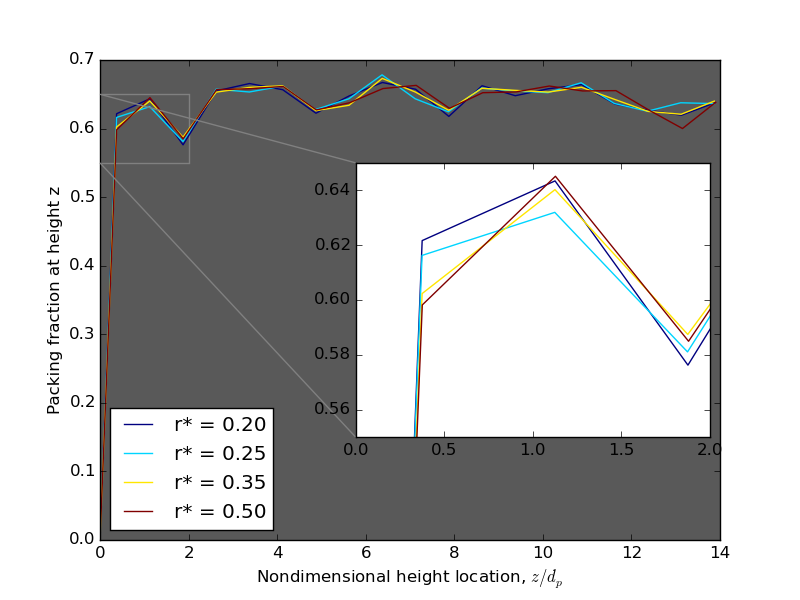
\includegraphics[width=\singleimagewidth]{chapters/figures/crush-fragments/packing-fraction-height.png}
    \caption{For only 1\% of crushed pebbles, the re-settling of small pebble fragments has a small effect on the overall packing fraction of the pebble bed. In the inset, the main influence is seen in the slight increase of packing fraction within the first pebble radius of the floor.}
    \label{fig:fragment-packing-fraction}
\end{figure}

From Fig.~\ref{fig:displacement-scatter}, the impression then arises that the large displacement magnitudes of the small crush fragments would result in an overall less-dense bed with large increase in packing fraction near the floor where pebbles settle. For 1\% crushed pebbles, there is some observable changes to the local packing fraction near the floor of the pebble bed, but no appreciable changes elsewhere in the bulk. In Fig.~\ref{fig:fragment-packing-fraction}, the packing fractions of the four different pebble beds are given. We look closely at the distribution within the first pebble diameter (see inset of Fig.~\ref{fig:fragment-packing-fraction}) and see the small crush fragments have a small change to the local packing fraction as they settled onto the floor of the container. Simulations can be run with a greater percentage of failed pebbles to discern more clearly the settling impact on local packing fractions. This is discussed in the Remaining Work section.


\begin{figure}[!ht]
	\centering
	\begin{subfigure}[b]{\doubleimagewidth}
		\centering
		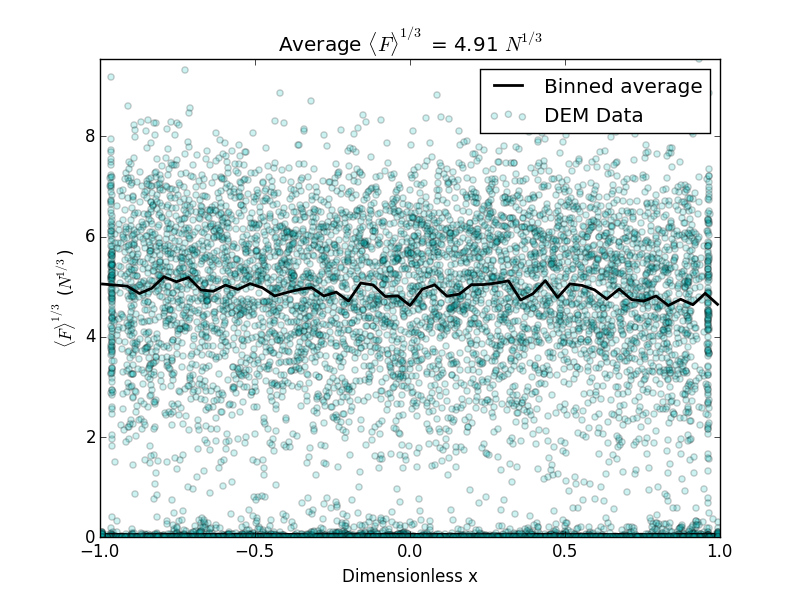
\includegraphics[width=\textwidth]{chapters/figures/crush-fragments/force-scatter-20.png}
		\caption{$r_1^* = 0.20$}\label{fig:fragment-contact-forces-20}
	\end{subfigure}
	\begin{subfigure}[b]{\doubleimagewidth}
		\centering
		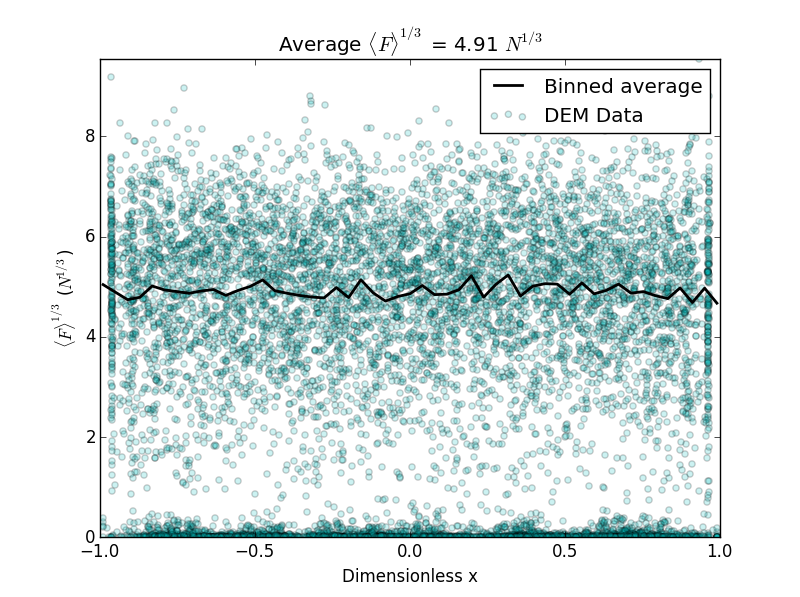
\includegraphics[width=\textwidth]{chapters/figures/crush-fragments/force-scatter-25.png}
		\caption{$r_1^* = 0.25$}\label{fig:fragment-contact-forces-25}
	\end{subfigure}

	\begin{subfigure}[b]{\doubleimagewidth}
		\centering
		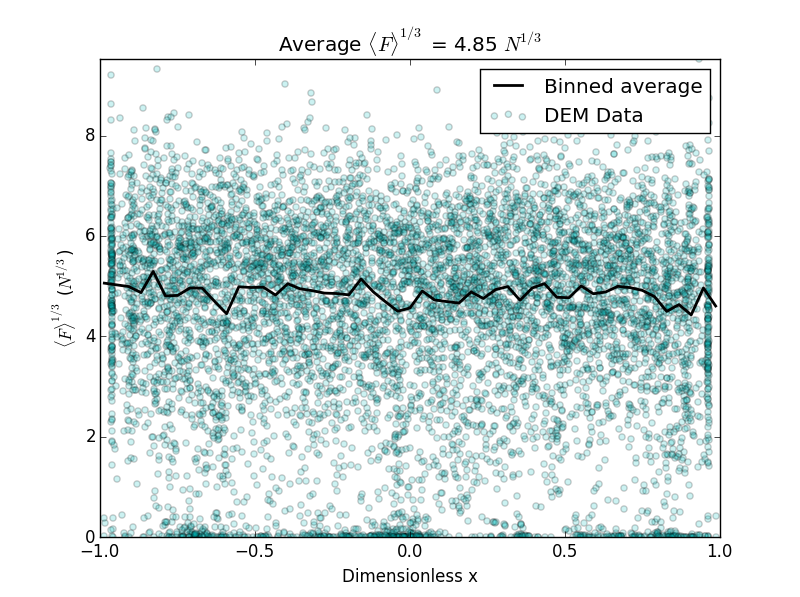
\includegraphics[width=\textwidth]{chapters/figures/crush-fragments/force-scatter-35.png}
		\caption{$r_1^* = 0.35$}
	\end{subfigure}
	\begin{subfigure}[b]{\doubleimagewidth}
		\centering
		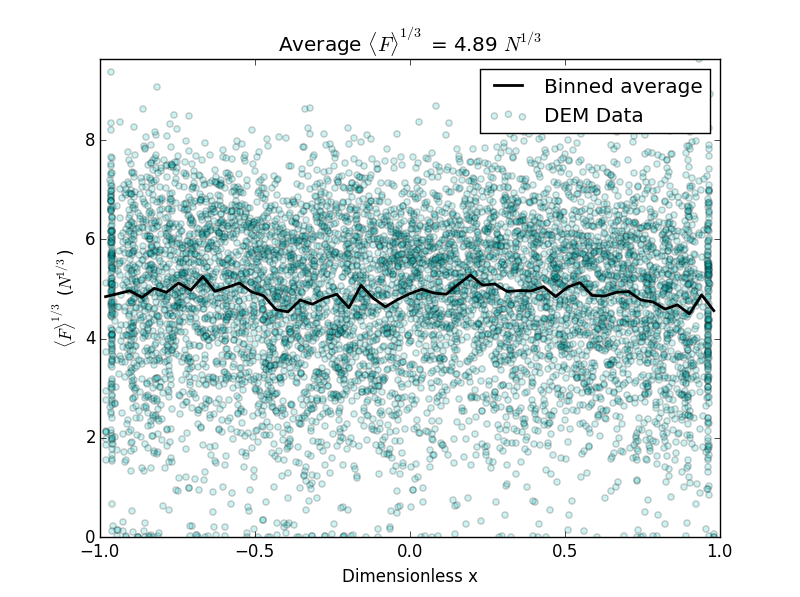
\includegraphics[width=\textwidth]{chapters/figures/crush-fragments/force-scatter-50.png}
		\caption{$r_1^* = 0.50$}
	\end{subfigure}
	\caption{Contact force distributions throughout the pebble beds with different crush fragment sizes. Average forces in the bed are largely unaffected by the size of crushed particle fragments.}
\label{fig:fragment-contact-forces}
\end{figure}

\FloatBarrier

The last point to discuss is how the different size particles change the distribution of contact forces inside the ensemble. We plot the scatter of contact forces for all the pebbles in the ensemble in Fig.~\ref{fig:fragment-contact-forces}. We are most interested in the contact loads carried by the large particles that make up the force network after crush fragments are inserted into the ensemble. The small fragments, moving through the interstitial gaps, are not expected to carry much load. Therefore in the data processing for the subplot of Figs.~\ref{fig:fragment-contact-forces-20} and~\ref{fig:fragment-contact-forces-25}, I did not include the vast number of small forces on the fragments in the average value of contact force. Opposingly, the larger fragments, $r_1^*>0.4$, are expected to be inserted firmly into the contact network and their contribution to the average value is included.

What we see in Fig.~\ref{fig:fragment-contact-forces} is that the average contact forces in the pebble bed remain mostly unchanged as a function of the size of the fragment radii. For all pebble beds, after the bed re-settles from the crushing event, the average contact forces (to the 1/3 power, which is the value important for heat transfer, see \cref{sec:dem-studies-effective-conductivity}) are approximately $4.9\ N^{1/3}$. None of the beds have a maximum value greater than $9\ N^{1/3}$.

\subsection{Conclusions of Pebble Failure Modeling}
[complete this!!!]
In this section I introduced a method for introducing crushed pebble fragments into an ensemble after a pebble is damaged. The method was necessary to conserve mass between pebble beds before and after the crushing event which is necessary for also balancing the energy deposition into the bed from volumetric heating before and after the crushing event. We then showed that fragments increase the computational time as $(1/r_1^*)^{1/3}$ while the necessary minimum volume for inserting the particles follows roughly as $(r_1^*)^{1/3}$. For the optimization of fragment size, the most important feature is to represent realistic physics. From this point of view, disrupting the packing with a large fragments is least desirable. Therefore, from the plot of Fig.~\ref{fig:volume-ratio}, we somewhat arbitrarily recommend fragments of size $r_1^* < 0.4$ to keep the required volume small. In terms of computation time, now as a secondary concern, we recommend fragments of size $r_1^* > 0.3$; keeping in mind as computer power and ease of parallelizing increases every year, this recommendation can quickly be relaxed to smaller fragment sizes.

The size of fragments may still influence the overall transport of energy in the system but in terms of localizing heat deposition due to settling fragments in interstitial regions, we showed that the local packing fraction was changed very little over the range of radius ratios we tested. Thus from the point of view of capturing proper thermo-physics of the system, there does not seem to be a strict sensitivity to choice of radius ratio. 